% ============================================================
% CCL FIGURES — LaTeX/TikZ Source
% A Conservation Law for Commitment in Language
% Deric J. McHenry / Ello Cello LLC
% Patent pending Serial No. 63/877,177
% DOI: 10.5281/zenodo.18792459
%
% Compile with: pdflatex ccl_figures.tex
% Requires: pgfplots, tikz, xcolor, amsmath
% ============================================================

\documentclass[10pt]{article}
\usepackage{geometry}
\geometry{margin=1.2in}
\usepackage{tikz}
\usepackage{pgfplots}
\pgfplotsset{compat=1.18}
\usepackage{xcolor}
\usepackage{amsmath}
\usepackage{caption}
\usepackage{subcaption}
\usepackage{float}
\usepackage{booktabs}

% --- Color definitions ---
\definecolor{ccl-red}{RGB}{192,57,43}
\definecolor{ccl-blue}{RGB}{36,113,163}
\definecolor{ccl-teal}{RGB}{26,138,101}
\definecolor{ccl-drift}{RGB}{160,40,20}
\definecolor{ccl-compress}{RGB}{30,90,160}
\definecolor{ccl-conserve}{RGB}{20,130,90}
\definecolor{ccl-gain-low}{RGB}{180,160,60}
\definecolor{ccl-gain-high}{RGB}{80,200,60}

\begin{document}

% ============================================================
% FIGURE L1 — Stability Curves
% ============================================================

\begin{figure}[H]
\centering
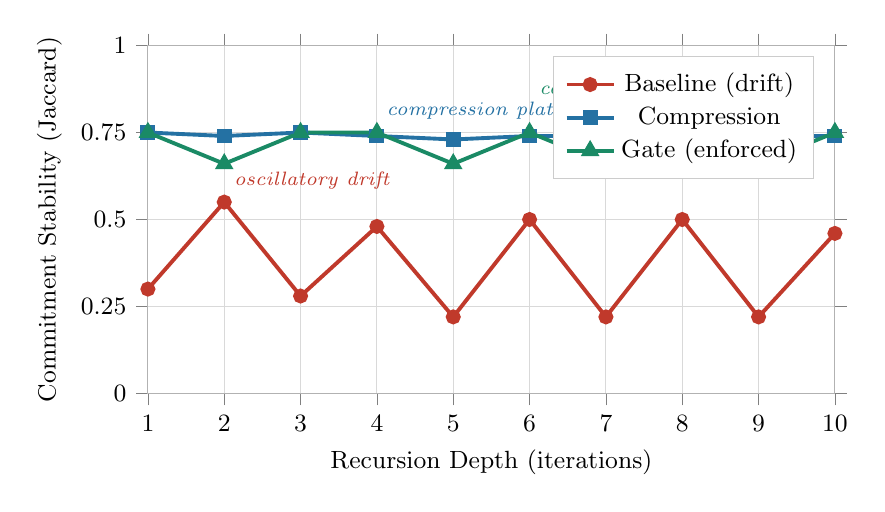
\begin{tikzpicture}
\begin{axis}[
  width=0.85\textwidth,
  height=6cm,
  xlabel={Recursion Depth (iterations)},
  ylabel={Commitment Stability (Jaccard)},
  xmin=1, xmax=10,
  ymin=0, ymax=1.0,
  xtick={1,2,3,4,5,6,7,8,9,10},
  ytick={0,0.25,0.5,0.75,1.0},
  yticklabel style={font=\small},
  xticklabel style={font=\small},
  xlabel style={font=\small},
  ylabel style={font=\small},
  grid=both,
  grid style={line width=0.3pt, draw=gray!20},
  major grid style={line width=0.4pt, draw=gray!30},
  legend pos=north east,
  legend style={font=\small, draw=gray!40, fill=white, inner sep=4pt},
  tick align=outside,
  axis line style={gray!60},
  clip=false,
]

% Baseline — oscillatory drift
\addplot[
  color=ccl-red,
  line width=1.4pt,
  mark=*,
  mark size=2pt,
  mark options={fill=ccl-red},
] coordinates {
  (1,0.30)(2,0.55)(3,0.28)(4,0.48)(5,0.22)(6,0.50)(7,0.22)(8,0.50)(9,0.22)(10,0.46)
};
\addlegendentry{Baseline (drift)}

% Compression — mid plateau
\addplot[
  color=ccl-blue,
  line width=1.4pt,
  mark=square*,
  mark size=2pt,
  mark options={fill=ccl-blue},
] coordinates {
  (1,0.75)(2,0.74)(3,0.75)(4,0.74)(5,0.73)(6,0.74)(7,0.74)(8,0.73)(9,0.74)(10,0.74)
};
\addlegendentry{Compression}

% Gate/enforcement — conservation
\addplot[
  color=ccl-teal,
  line width=1.4pt,
  mark=triangle*,
  mark size=2.5pt,
  mark options={fill=ccl-teal},
] coordinates {
  (1,0.75)(2,0.66)(3,0.75)(4,0.75)(5,0.66)(6,0.75)(7,0.66)(8,0.75)(9,0.66)(10,0.75)
};
\addlegendentry{Gate (enforced)}

% Regime annotations
\node[font=\scriptsize\itshape, text=ccl-red, anchor=south west]
  at (axis cs:2,0.56) {oscillatory drift};
\node[font=\scriptsize\itshape, text=ccl-blue, anchor=south west]
  at (axis cs:4,0.76) {compression plateau};
\node[font=\scriptsize\itshape, text=ccl-teal, anchor=south west]
  at (axis cs:6,0.82) {conservation regime};

\end{axis}
\end{tikzpicture}
\caption{
  \textbf{Commitment Stability Across Recursive Transformation.}
  Mean Jaccard stability over 10 recursive iterations across $n=20$
  commitment-bearing signals. Three regimes: \textit{baseline}
  (unmediated transformation) exhibits oscillatory drift consistent
  with entropic decay under recursive load; \textit{compression}
  stabilizes at an intermediate plateau ($\approx 0.74$), reducing
  variance without full conservation; \textit{gate/enforcement}
  sustains highest stability, consistent with $\mathcal{C}(T(S)) \approx \mathcal{C}(S)$.
  The enforcement premium — marginal conservation beyond compression
  alone — is visible as the gap between the upper two curves.
  Data: \texttt{corpus\_run\_20260317}, \texttt{convergence\_v2\_234059}.
}
\label{fig:L1-stability}
\end{figure}

\clearpage

% ============================================================
% FIGURE E1 — Fidelity Heatmap (as grouped bar chart for LaTeX)
% ============================================================

\begin{figure}[H]
\centering
\begin{tikzpicture}
\begin{axis}[
  width=0.88\textwidth,
  height=10cm,
  xbar,
  bar width=5pt,
  xlabel={Jaccard Fidelity Score},
  xmin=0, xmax=1.1,
  xtick={0,0.25,0.5,0.75,1.0},
  xticklabel style={font=\scriptsize},
  yticklabel style={font=\scriptsize},
  xlabel style={font=\small},
  ytick=data,
  yticklabels={
    specification, legal, conditional, obligation, regulation,
    mandate, code, constraint, contractual, requirement,
    protocol, standard, agreement, instructional, directive,
    policy, procedural, prohibition, definition, rule
  },
  y dir=normal,
  enlarge y limits={abs=8pt},
  legend style={
    at={(0.98,0.02)},
    anchor=south east,
    font=\small,
    draw=gray!40,
  },
  grid=x,
  grid style={line width=0.3pt, draw=gray!20},
  axis line style={gray!60},
  tick align=outside,
]

% Baseline bars
\addplot[
  xbar,
  fill=ccl-blue!60,
  draw=ccl-blue!80,
  bar width=4pt,
] coordinates {
  (0.287,1)(0.713,2)(0.729,3)(0.408,4)(0.327,5)
  (0.833,6)(0.389,7)(0.500,8)(0.733,9)(0.731,10)
  (0.750,11)(0.750,12)(0.774,13)(0.857,14)(0.857,15)
  (0.524,16)(0.000,17)(0.000,18)(0.000,19)(0.000,20)
};
\addlegendentry{Baseline}

% Enforcement bars
\addplot[
  xbar,
  fill=ccl-teal!70,
  draw=ccl-teal!90,
  bar width=4pt,
] coordinates {
  (0.583,1)(1.000,2)(1.000,3)(0.667,4)(0.583,5)
  (1.000,6)(0.556,7)(0.667,8)(0.818,9)(0.817,10)
  (0.817,11)(0.815,12)(0.823,13)(0.906,14)(0.906,15)
  (0.573,16)(0.000,17)(0.000,18)(0.000,19)(0.000,20)
};
\addlegendentry{Enforcement}

\end{axis}
\end{tikzpicture}
\caption{
  \textbf{Commitment Fidelity by Signal Category.}
  Jaccard fidelity scores under baseline (unmediated) and enforcement
  conditions across $n=20$ signal categories, recursion depth $=20$.
  Categories are sorted by enforcement gain $\Delta$.
  Highest gains: specification ($+0.297$), legal ($+0.287$),
  conditional ($+0.271$), obligation ($+0.258$), regulation ($+0.257$).
  Categories at the stability ceiling (procedural, prohibition, rule,
  definition) show fidelity $= 0$ under both conditions, a known
  artifact of high-density canonical forms under compression.
  Mean fidelity gain across corpus: $+0.118$ ($n=20$).
  Source: \texttt{corpus\_run\_20260317\_085833}.
}
\label{fig:E1-fidelity}
\end{figure}

\clearpage

% ============================================================
% FIGURE L2 — Phase Surface (conceptual, using pgfplots surf)
% ============================================================

\begin{figure}[H]
\centering
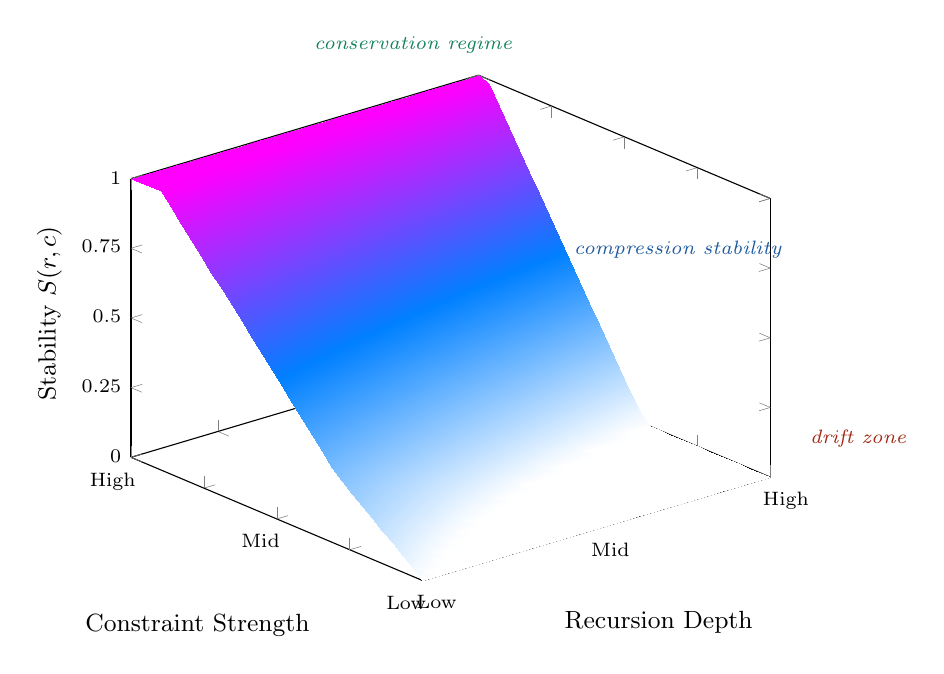
\begin{tikzpicture}
\begin{axis}[
  width=0.80\textwidth,
  height=8cm,
  xlabel={Recursion Depth},
  ylabel={Constraint Strength},
  zlabel={Stability $S(r,c)$},
  xlabel style={font=\small},
  ylabel style={font=\small},
  zlabel style={font=\small},
  xmin=0, xmax=1,
  ymin=0, ymax=1,
  zmin=0, zmax=1,
  xtick={0,0.25,0.5,0.75,1},
  ytick={0,0.25,0.5,0.75,1},
  ztick={0,0.25,0.5,0.75,1},
  xticklabels={Low,,Mid,,High},
  yticklabels={Low,,Mid,,High},
  xticklabel style={font=\scriptsize},
  yticklabel style={font=\scriptsize},
  zticklabel style={font=\scriptsize},
  view={-40}{30},
  colormap/cool,
  surf,
  shader=interp,
  samples=30,
  domain=0:1,
  y domain=0:1,
  mesh/cols=30,
]

% Surface: S(r,c) = c*0.85 - (1-c)*r*0.7 + max(0, (c-0.3))*0.4*(1-r*0.3)
% Clamped to [0,1]
\addplot3[
  surf,
  shader=interp,
  colormap/cool,
  samples=30,
  domain=0:1,
  y domain=0:1,
] { max(0, min(1,
    y*0.85
    - (1-y)*x*0.70
    + max(0,(y-0.3))*0.40*(1-x*0.30)
  ))
};

\end{axis}

% Regime labels (positioned via node in tikzpicture coords)
\node[font=\scriptsize\itshape, text=ccl-drift, anchor=west]
  at (8.5,1.8) {drift zone};
\node[font=\scriptsize\itshape, text=ccl-compress, anchor=west]
  at (5.5,4.2) {compression stability};
\node[font=\scriptsize\itshape, text=ccl-conserve, anchor=west]
  at (2.2,6.8) {conservation regime};

\end{tikzpicture}
\caption{
  \textbf{Commitment Stability Phase Surface.}
  Stability $S(r,c)$ as a joint function of recursion depth $r$ and
  constraint strength $c$. Three structural regimes: the
  \textit{drift zone} (low $c$, high $r$) where
  $\mathcal{C}(T^n(S)) \ll \mathcal{C}(S)$; the
  \textit{compression stability} band (intermediate $c$) where
  surface stabilization occurs without full conservation; and the
  \textit{conservation regime} (strong $c$, any $r$) where
  $\mathcal{C}(T^n(S)) \approx \mathcal{C}(S)$.
  The stability basin forms a ridge orthogonal to the recursion
  axis, constituting a structural invariant under recursive load.
  This figure is conceptual; the surface function is a structural
  analog of the empirical regime signatures in Figure~\ref{fig:L1-stability}.
}
\label{fig:L2-phase}
\end{figure}

\end{document}

% ============================================================
% USAGE NOTES
% ============================================================
%
% 1. To compile:
%    pdflatex ccl_figures.tex
%    (run twice for cross-references)
%
% 2. Required packages:
%    - pgfplots (>= 1.18)
%    - tikz
%    - xcolor
%    - amsmath
%    - caption, subcaption, float, booktabs
%
% 3. To include individual figures in your main paper:
%    Copy the \begin{figure}...\end{figure} blocks into your
%    paper .tex file. Colors and packages must be defined in the
%    preamble of the main file.
%
% 4. For Figure L2 (3D surface), if compile is slow:
%    Reduce samples=30 to samples=20 for draft mode.
%    Restore to samples=40+ for final submission.
%
% 5. arXiv submission:
%    Include this .tex file + no external images needed.
%    All figures are generated inline by pgfplots/TikZ.
%    arXiv will compile the .tex directly.
%
% 6. Citation block for captions:
%    Patent pending Serial No. 63/877,177
%    DOI: https://doi.org/10.5281/zenodo.18792459
%    \copyright 2026 Ello Cello LLC. All rights reserved.
%
% ============================================================
